% planisphere.tex
%
% The LaTeX code in this file brings together into a single document the
% various components of the model planisphere.
%
% Copyright (C) 2014-2020 Dominic Ford <dcf21-www@dcford.org.uk>
%
% This code is free software; you can redistribute it and/or modify it under
% the terms of the GNU General Public License as published by the Free Software
% Foundation; either version 2 of the License, or (at your option) any later
% version.
%
% You should have received a copy of the GNU General Public License along with
% this file; if not, write to the Free Software Foundation, Inc., 51 Franklin
% Street, Fifth Floor, Boston, MA  02110-1301, USA

% ----------------------------------------------------------------------------

\documentclass[a4paper,onecolumn,10pt]{article}
\usepackage[dvips]{graphicx}
\usepackage{fancyhdr,url}
\usepackage{parskip}
\usepackage[pdftitle={Build your own planisphere}, pdfauthor={Dominic Ford}, pdfsubject={Build your own planisphere}, pdfkeywords={Build your own planisphere}, colorlinks=true, linkcolor=blue, citecolor=blue, filecolor=blue, urlcolor=blue]{hyperref}
\renewcommand{\familydefault}{\sfdefault}
\pagestyle{fancy}

\lhead{\it MAKE YOUR OWN PLANISPHERE}
\chead{}
\rhead{\thepage}
\lfoot{}\rfoot{}
\cfoot{\bf\footnotesize\copyright\ 2014--2020 Dominic Ford. Distributed under the GNU General Public License, version 3. Document downloaded from \url{https://in-the-sky.org/planisphere/}}

\fancypagestyle{plain}{%
\fancyhf{} % clear all header and footer fields
\renewcommand{\headrulewidth}{0pt}
\renewcommand{\footrulewidth}{0pt}}

\title{Make your own planisphere}
\author{Dominic Ford}
\date{2014--2020}

\begin{document}
\maketitle
\setcounter{footnote}{1}

A planisphere is a simple hand-held device which shows a map of which stars are
visible in the night sky at any particular time. By rotating a wheel, it shows
how stars move across the sky through the night, and how different
constellations are visible at different times of year.

Here, I present a kit which you can download and print to make your own
planisphere out of paper or cardboard.

The design of a planisphere depends on the geographic location where it is to
be used, since different stars are visible from different places. I have
created kits for use at a wide range of latitudes, which you can download from

\url{https://in-the-sky.org/planisphere/}

The planisphere presented in this document is designed for use at a latitude of
\input{tmp/lat}.
 
\section*{What you need}

\begin{itemize}
\item Two sheets of A4 paper, or preferably thin card.
\item Scissors.
\item A split-pin fastener.
\item Optional: one sheet of transparent plastic, e.g. acetate designed for use with overhead projectors.
\item Optional: A little glue.
\end{itemize}

\section*{Assembly instructions}

{\bf Step 1} -- Planispheres look slightly different depending on where you
live. The planisphere prepared in this document is designed for use anywhere on
Earth which is within a few degrees of latitude \input{tmp/lat}. If you live
elsewhere, you should download an alternative kit from

\url{https://in-the-sky.org/planisphere/}

{\bf Step 2} -- Print the pages at the back of this PDF file, showing the
star wheel and the body of the planisphere, onto two separate sheets of paper,
or more preferably onto thin card.

{\bf Step 3} -- Carefully cut out the star wheel and the body of the
planisphere. Also cut out the shaded grey area of the planisphere's body, and
if you have it, the grid of lines which you have printed onto transparent
plastic. If you are using cardboard, you may wish to carefully score the body
of the planisphere along the dotted line to make it easier to fold it along
this line later.

{\bf Step 4} -- The star wheel has a small circle at its center, and the
planisphere's body has a matching small circle at the bottom. Make a small hole
(about 2mm across) in each. If a paper drill is to hand, these are ideal,
otherwise use a compass point and enlarge the hole by turning in a circular
motion.

{\bf Step 5} -- Slot a split-pin fastener through the middle of the
star wheel, with the head of the fastener against the printed side of the
star wheel. Then slot the body of the planisphere onto the same fastener, with
the printed side facing the back of the fastener. Fold the fastener down to
secure the two sheets of cardboard together.

{\bf Step 6 (Optional)} -- If you printed the final page of the PDF file
onto a sheet of plastic, you should now stick this grid of lines over the
viewing window which you cut out from the body of the planisphere.

{\bf Step 7} -- Fold the body of the planisphere along the dotted line,
so that the front of the star wheel shows through the window which you cut in
the body.

{\bf Congratulations, your planisphere is now ready for use!}

\section*{How to use your planisphere}

Turn the star wheel until you find the point around its edge where today's date
is marked, and line this point up with the current time. The viewing window now
shows all of the constellations that are visible in the sky.

Go outside and face north. Holding the planisphere up to the sky, the stars
marked at the bottom of the viewing window should match up with those that you
see in the sky in front of you.

Turn to face east or west, and rotate the planisphere so that the word "East"
or "West" is at the bottom of the window. Once again, the stars at the bottom
of the viewing window should match up with those that you see in the sky in
front of you.

If you printed the grid of altitude and azimuth lines onto transparent plastic,
these lines let you work out how high objects will appear in the sky, and in
which direction. The circles are drawn at altitudes of 10, 20, 30, ..., 80
degrees above the horizon. For reference, a distance of ten degrees roughly
equates to a hand-span at arm's length. The curved lines are vertical lines
connecting points on the horizon up to the point immediately above your head.
They are drawn in the cardinal directions S, SSE, SE, ESE, E, etc.

\section*{Customised planispheres}

This planisphere kit was designed using a collection of Python scripts and the
pycairo graphics library. If you would like to customise your planisphere, you
are welcome to download the scripts from my GitHub account and modify them,
providing you credit the source:

\url{https://github.com/dcf21/planisphere}

\section*{License}

Like everything else on {\tt In-The-Sky.org}, these planisphere kits are
\copyright\ Dominic Ford. However, everything on {\tt In-The-Sky.org} is
provided for the benefit of amateur astronomers worldwide, and you are welcome
to modify and/or redistribute any of the material on this website, under the
following conditions: (1) Any item that has an associated copyright text {\bf
must} include that {\bf unmodified} text in your redistributed version, (2) You
{\bf must} credit me, Dominic Ford, as the original author and copyright
holder, (3) You {\bf may not} derive any profit from your reproduction of
material on this website, {\bf unless} you are a registered charity whose
express aim is the advancement of astronomical science, {\bf or} you have the
written permission of the author.

\newpage

\centerline{\includegraphics{tmp/starwheel}}

\vspace{1cm}
The planisphere's central star wheel, which should be sandwiched inside the folded holder.

\newpage
\thispagestyle{empty}
\vspace*{-3.0cm}
\centerline{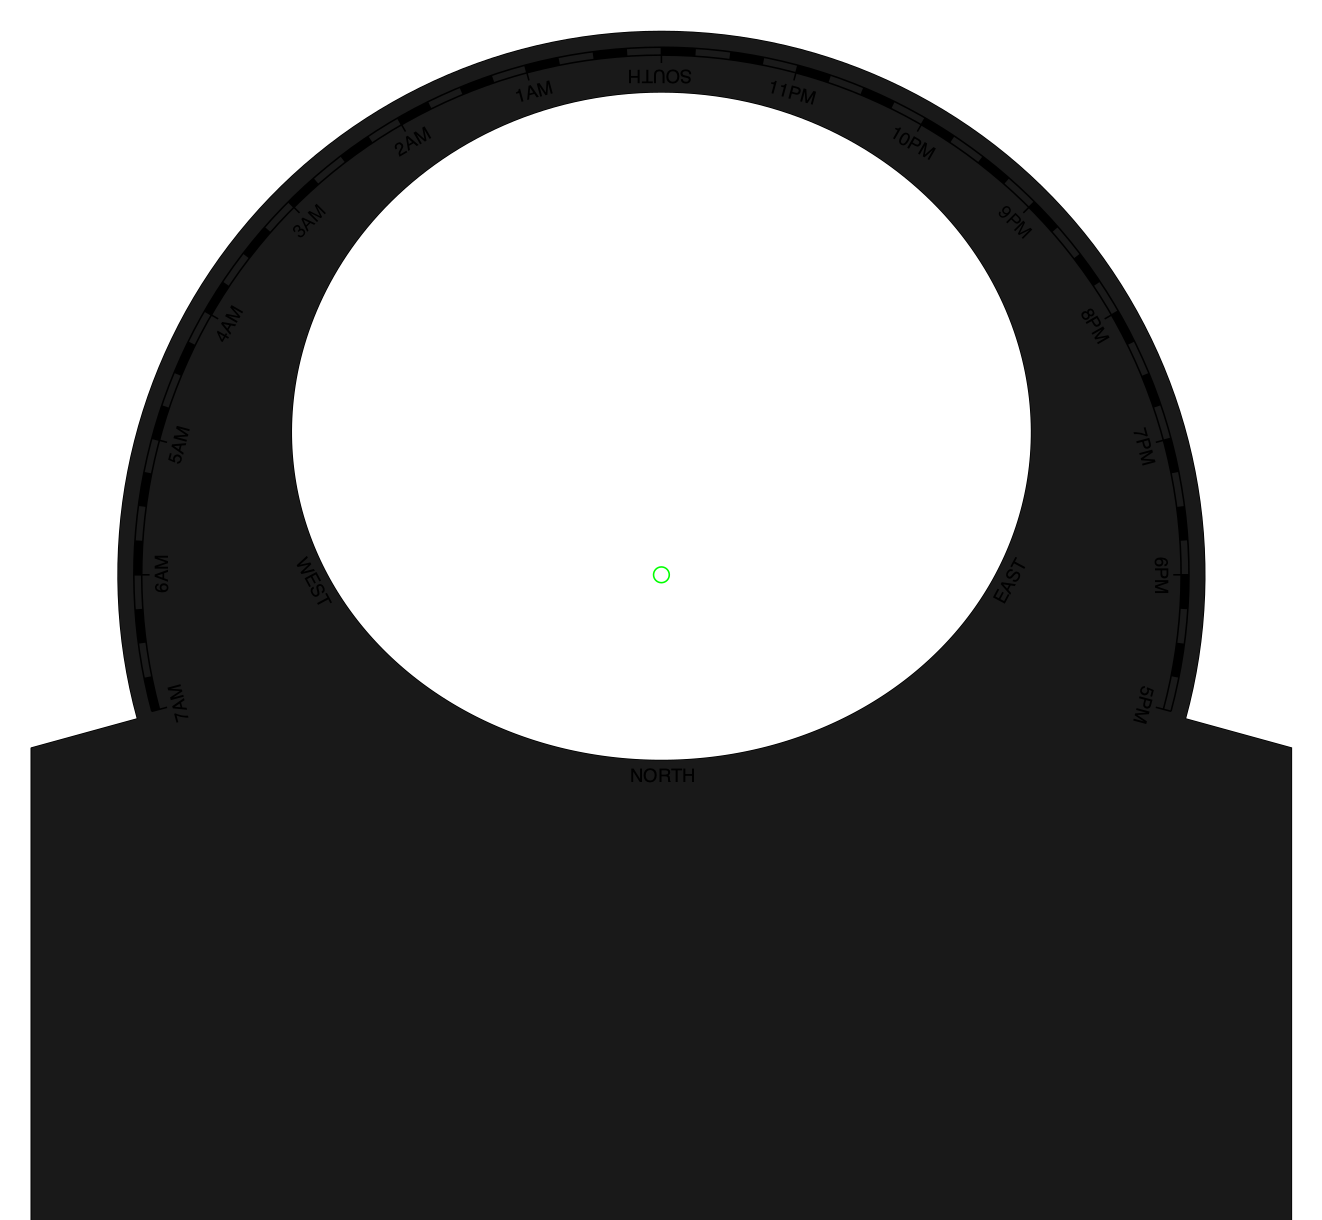
\includegraphics{tmp/holder}}
\newpage

\centerline{\includegraphics{tmp/altaz}}

\vspace{1cm}
This grid of lines can optionally be printed onto transparent plastic and glued into the cut out window in the planisphere's body to show the altitudes of objects in the sky, and their directions.

\end{document}

